\section{RTC::Data\-Flow\-Participant Interface Reference}
\label{interfaceRTC_1_1DataFlowParticipant}\index{RTC::DataFlowParticipant@{RTC::DataFlowParticipant}}
Execution\-Semantics::Data\-Flow\-Participant component.  


{\tt import \char`\"{}RTC.idl\char`\"{};}

Inheritance diagram for RTC::Data\-Flow\-Participant::\begin{figure}[H]
\begin{center}
\leavevmode
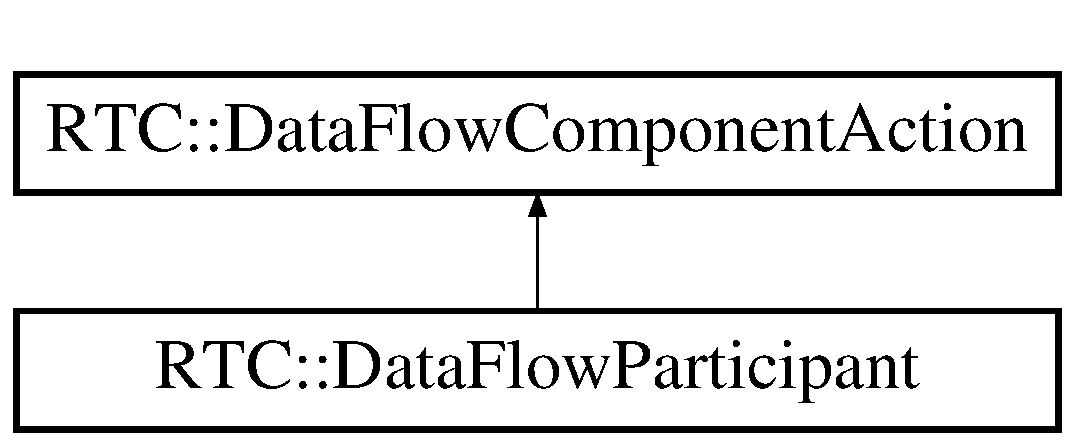
\includegraphics[height=2cm]{interfaceRTC_1_1DataFlowParticipant}
\end{center}
\end{figure}
\subsection*{Public Member Functions}
\begin{CompactItemize}
\item 
{\bf Return\-Code\_\-t} {\bf on\_\-execute} (in {\bf Unique\-Id} ec\_\-id)
\item 
{\bf Return\-Code\_\-t} {\bf on\_\-state\_\-update} (in {\bf Unique\-Id} ec\_\-id)
\item 
{\bf Return\-Code\_\-t} {\bf on\_\-rate\_\-changed} (in {\bf Unique\-Id} ec\_\-id)
\end{CompactItemize}


\subsection{Detailed Description}
Execution\-Semantics::Data\-Flow\-Participant component. 



\subsection{Member Function Documentation}
\index{RTC::DataFlowParticipant@{RTC::Data\-Flow\-Participant}!on_execute@{on\_\-execute}}
\index{on_execute@{on\_\-execute}!RTC::DataFlowParticipant@{RTC::Data\-Flow\-Participant}}
\subsubsection{\setlength{\rightskip}{0pt plus 5cm}{\bf Return\-Code\_\-t} RTC::Data\-Flow\-Component\-Action::on\_\-execute (in {\bf Unique\-Id} {\em ec\_\-id})\hspace{0.3cm}{\tt  [inherited]}}\label{interfaceRTC_1_1DataFlowComponentAction_RTC_1_1DataFlowParticipanta0}


\index{RTC::DataFlowParticipant@{RTC::Data\-Flow\-Participant}!on_rate_changed@{on\_\-rate\_\-changed}}
\index{on_rate_changed@{on\_\-rate\_\-changed}!RTC::DataFlowParticipant@{RTC::Data\-Flow\-Participant}}
\subsubsection{\setlength{\rightskip}{0pt plus 5cm}{\bf Return\-Code\_\-t} RTC::Data\-Flow\-Component\-Action::on\_\-rate\_\-changed (in {\bf Unique\-Id} {\em ec\_\-id})\hspace{0.3cm}{\tt  [inherited]}}\label{interfaceRTC_1_1DataFlowComponentAction_RTC_1_1DataFlowParticipanta2}


\index{RTC::DataFlowParticipant@{RTC::Data\-Flow\-Participant}!on_state_update@{on\_\-state\_\-update}}
\index{on_state_update@{on\_\-state\_\-update}!RTC::DataFlowParticipant@{RTC::Data\-Flow\-Participant}}
\subsubsection{\setlength{\rightskip}{0pt plus 5cm}{\bf Return\-Code\_\-t} RTC::Data\-Flow\-Component\-Action::on\_\-state\_\-update (in {\bf Unique\-Id} {\em ec\_\-id})\hspace{0.3cm}{\tt  [inherited]}}\label{interfaceRTC_1_1DataFlowComponentAction_RTC_1_1DataFlowParticipanta1}




The documentation for this interface was generated from the following file:\begin{CompactItemize}
\item 
{\bf RTC.idl}\end{CompactItemize}
